\documentclass[conference,compsoc]{IEEEtran}
%\documentclass[letterpaper]{sig-alternate-05-2015}

%------------------------------------------------------------------------------
%                                  Preamble.
%------------------------------------------------------------------------------
%
\usepackage{url}
% \usepackage{color}
\usepackage{wrapfig}
\usepackage{graphicx}
\usepackage{hyphenat}
\usepackage{xspace}
\usepackage{txfonts}
\usepackage[sort&compress]{natbib}
\newcommand{\subparagraph}{}
\usepackage[small,compact]{titlesec}
\usepackage[ruled,vlined]{algorithm2e}
\usepackage[pdftex,unicode=true,%
                   pdfstartview={FitH},%
                   colorlinks=true,%
                   citecolor=black,%
                   filecolor=black,%
                   linkcolor=black,%
                   urlcolor=black]{hyperref}

% Use a smaller font size for URLs:
\makeatletter
\def\url@myurlstyle{%
   \@ifundefined{selectfont}{\def\UrlFont{\tt}}{\def\UrlFont{\tt}}}
   \makeatother
\urlstyle{myurl}

% Section names, figure names and algorithm names.
\renewcommand{\tableautorefname}{Table}
\renewcommand{\figureautorefname}{Figure}
\renewcommand{\sectionautorefname}{Section}
\renewcommand{\subsectionautorefname}{Section}
\renewcommand{\subsubsectionautorefname}{Section}
\newcommand{\figref}[1]{\autoref{#1}}
\newcommand{\tabref}[1]{\autoref{#1}}
\newcommand{\sectref}[1]{\autoref{#1}}
\newcommand{\mycaption}[2]{\caption{#1}#2}
\newcommand{\myparagraphsquish}[1]{\noindent\textbf{\textit{#1}}}
\newcommand{\myparagraph}[1]{\parskip -4pt \indent\par\noindent\textbf{\textit{#1}} \parskip 0pt}
\newcommand{\myfootnote}[1]{\footnote{\scriptsize #1}}

%------------------------------------------------------------------------------
%                                Space savers.
%------------------------------------------------------------------------------
% This mylist environment indents items, and saves less space than the above.
\newcounter{myctr}
\newenvironment{mylist}{\begin{list}{(\textbf{\arabic{myctr}})}
{\usecounter{myctr}
\setlength{\topsep}{1mm}\setlength{\itemsep}{0.5mm}
\setlength{\parsep}{0.5mm}
\setlength{\listparindent}{\parindent} % Indentation of paras.
\setlength{\itemindent}{0mm}\setlength{\partopsep}{0mm}
\setlength{\labelwidth}{-2mm}
\setlength{\leftmargin}{0mm}}}{\end{list}}

% Space saving List environment for itemizing.
\newenvironment{mybullet}{\begin{list}{$\bullet$}
{\setlength{\topsep}{1mm}\setlength{\itemsep}{0.5mm}
\setlength{\parsep}{0.5mm}
\setlength{\listparindent}{\parindent} % Indentation of paras.
\setlength{\itemindent}{0mm}\setlength{\partopsep}{0mm}
\setlength{\labelwidth}{-2mm}
\setlength{\leftmargin}{0mm}}}{\end{list}}

%------------------------------------------------------------------------------
%                  Useful commands and acronymns used in the paper.
%------------------------------------------------------------------------------
% Commands
\newcommand{\mycomment}[1]{}
\newcommand{\todo}[1]{\textcolor{red}{\textit{\textbf{!!!#1!!!}}}}
\newcommand{\CT}{\todo{\cite{TODO}}}

% Acronymns
\newcommand{\code}[1]{{\tt \footnotesize #1}}
\newcommand{\tab}{~~~~~}
\newcommand{\apriori}{\textit{a priori}}
\newcommand{\etal}{\textit{et al.}\xspace}
\newcommand{\eg}{\textit{e.g.,}\xspace}
\newcommand{\ie}{\textit{i.e.,}\xspace}
\newcommand{\adhoc}{ad hoc}

% Paper-specific acronyms
\newcommand{\tool}{EnGarde\xspace} % Client enclave code inspection library.
\newcommand{\TOOL}{EnGarde\xspace} % Client enclave code inspection library.

% Paper setup
\pdfpagewidth=8.5in
\pdfpageheight=11in

%------------------------------------------------------------------------------
%                               Fancy header setup.
%------------------------------------------------------------------------------
%
% \pagestyle{fancyplain}
% \lhead{}
% \lfoot{}
% \chead{}
% \rhead{}
% \cfoot{\thepage}
% \rfoot{}
% \renewcommand{\headrulewidth}{0pt}

%------------------------------------------------------------------------------
%                              Title and Authors.
%------------------------------------------------------------------------------
\begin{document}

\title{\tool: Mutually-Trusted Inspection of SGX Enclaves}
\author{Hai Nguyen and Vinod Ganapathy\\
Department of Computer Science, Rutgers University\\
\{hdn11, vinodg\}@cs.rutgers.edu}

\maketitle
%------------------------------------------------------------------------------
%                                  Abstract.
%------------------------------------------------------------------------------
\begin{abstract}
%
Smart personal devices equipped with a wide range of sensors and peripherals
can potentially be misused in various environments. They can be used to
exfiltrate sensitive information from enterprises and federal offices or be
used to smuggle unauthorized information into classrooms and examination halls.
One way to prevent these situations is to regulate how smart devices are used
in such restricted spaces. In this paper, we present an approach that robustly
achieves this goal for ARM TrustZone-based personal devices. In our approach,
restricted space hosts use remote memory operations to analyze and regulate
guest devices within the restricted space. We show that the ARM TrustZone
allows our approach to obtain strong security guarantees while only requiring a
small trusted computing base to execute on guest devices.

%
\end{abstract}

%------------------------------------------------------------------------------
%                                Main Contents.
%------------------------------------------------------------------------------

\section{Introduction}
\label{section:introduction}

Over the last several years, we have witnessed a number of advances in mobile
computing technology. Mobile devices are now available in a variety of form
factors, such as glasses, watches, smartphones, tablets, personal robots, and
even cars. These devices come equipped with powerful processors, ample storage,
and a diverse array of sensors. Coupled with advances in operating systems and
middleware for mobile devices, programmers can now avail rich programming APIs
to build software (``\textit{apps}'') that leverage these advances in hardware.
Modern app markets contain hundreds of thousands of apps, and the number and
diversity of apps available to end-users has further contributed to the
popularity of mobile devices. These advances in hardware and software have made
mobile devices viable replacements for desktop computers.

At the same time, we are also witnessing a fundamental shift in the practice of
software development due largely to the dynamics of mobile app development.
Until a few years ago, the task of developing software (targeting mainly
desktop computers) was mostly confined to teams of software engineers, either
in the open-source community or at IT companies. In contrast, it is common even
for individuals or small teams to build and distribute software via mobile app
markets. Such teams, or individuals, may lack the expertise and experience of a
large team of developers and often face economic and time constraints during
app development.  Nevertheless, mobile app development teams aim to maximize
revenue by making their apps available on a wide variety of mobile devices,
\ie~those running software stacks such as Android, iOS, and Windows. Apps that
are available for a wide variety of mobile devices can reach a large user base,
and can therefore generate more revenue either through app purchases or via
in-app advertisements.

One way to build apps for different mobile platforms is to create customized
versions of apps for each platform, \eg~a separate version of the app for
Android, iOS and Windows devices. However, this approach leads to multiple
versions of the app's code-base, which are difficult to maintain and evolve
over time. Moreover, this approach is poorly-suited for small mobile app
development teams, which must now dedicate resources to create, maintain and
evolve different versions of the app for each mobile platform.

As a result of these shortcomings, developers are increasingly adopting
\textit{cross-platform mobile app development frameworks}. These frameworks
allow developers to program the app's logic once in a high-level language, and
provide tool-support to allow the app to execute on a number of mobile
platforms. 

\begin{figure*}[t!]
\centering
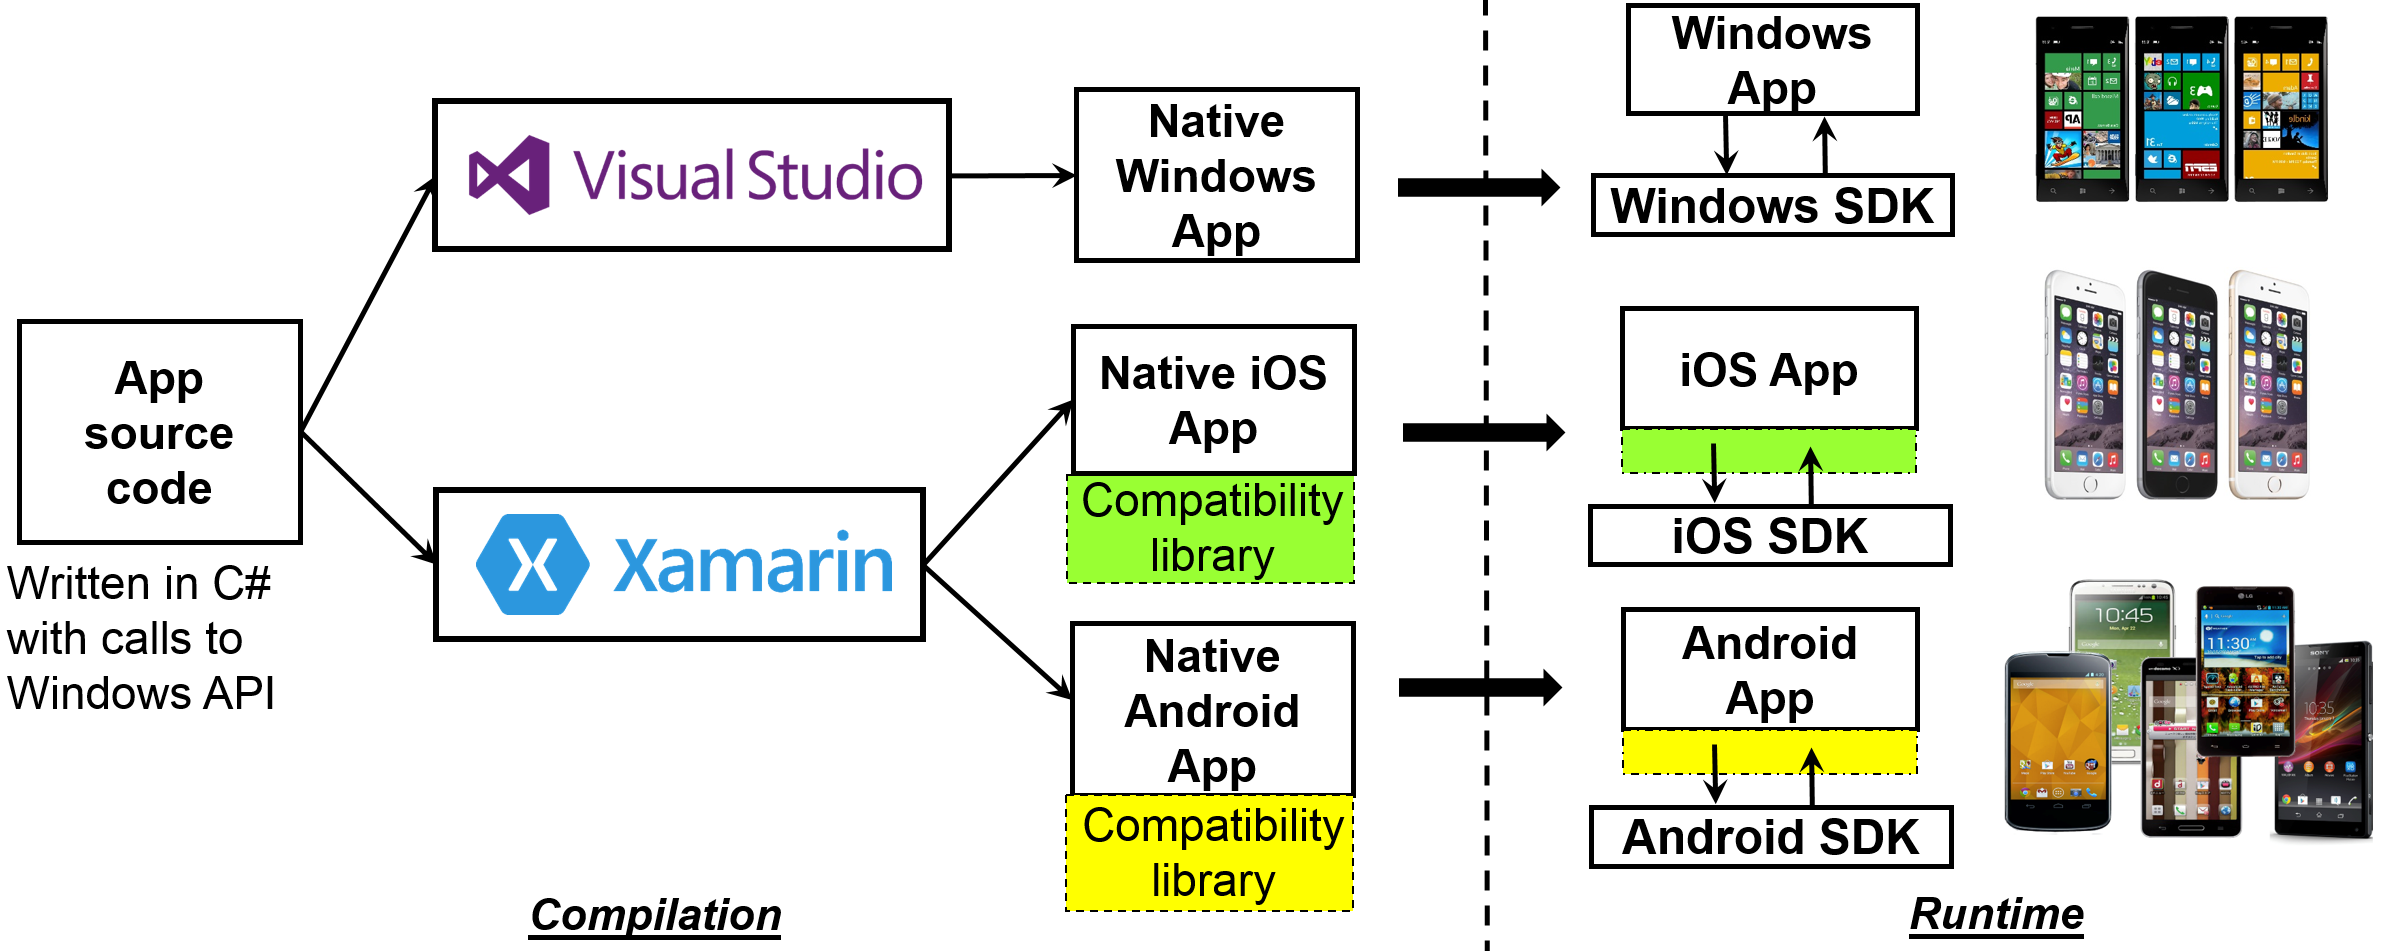
\includegraphics[keepaspectratio=true,width=0.9\textwidth]{figures/xptools-overview.png}
\mycaption{Overall operation of a cross-platform mobile app development
framework, using Xamarin as a concrete example. Developers build apps as they
would for the Windows Phone, in C\# using calls to the API of the Windows Phone
SDK. This code can directly be compiled to Windows Phone apps using the Visual
Studio toolchain. Xamarin allows developers to use the same source code to
build native Android or iOS apps. Xamarin provides compatibility libraries
that translate Windows SDK API calls in the code to the relevant API calls of
the underlying Android and iOS SDKs.}{\label{figure:xplatform-overview}}
\end{figure*}

There are two broad classes of cross-platform frameworks available today.  The
first class, which we call \textit{Web-based frameworks}, allows developers to
build mobile apps using languages popularly used to build Web applications,
such as HTML5, JavaScript, and CSS. Examples of such frameworks include Adobe
PhoneGap~\cite{phonegap}, Sencha~\cite{sencha} and IBM
MobileFirst~\cite{worklight}.  Developers specify the app's logic and user
interface using one or more of the Web-development languages.  However, these
languages do not contain primitives to allow apps to access resources on the
phone, \eg~peripherals such as the camera and microphone, the address book, and
phone settings. Thus, Web-based frameworks provide supporting runtime libraries
that end-users must download and execute on their mobile devices. Mobile apps
interface with these libraries to access resources on the mobile devices---such
mobile apps are also popularly called hybrid mobile apps.  Web-based frameworks
allow developers to rapidly prototype mobile apps.  However, these frameworks
are ill-suited for high-performance apps, such as games or those that use
animation. The expressiveness of the resulting mobile apps is also limited by
the interface exported by the runtime libraries offered by the frameworks.


The second class, which we call \textit{native frameworks}, addresses the above
challenges. Examples of such frameworks include Xamarin~\cite{xamarin},
Apportable~\cite{apportable} and MD$^2$~\cite{md2:sac13,myappconverter}. These
frameworks generally support a \textit{home platform} and one or more
\textit{target platforms}. Developers build mobile apps as they normally would
for the home platform, and leverage the framework's support to automatically
produce apps for the target platforms as well. For example, the home platform
for Xamarin is Windows Phone, and developers build apps using C\# and the API
of the Windows Phone SDK. The Xamarin framework allows developers to
automatically build Android and iOS apps using this code base (see
\figref{figure:xplatform-overview}). Likewise, the home platform for Apportable
is iOS. Developers build apps using Objective-C and the iOS SDK, and leverage
Apportable to produce Android apps from this code base.  In this paper, we will
focus on native frameworks for cross-platform mobile app development. 

When an app developer uses native frameworks, he implicitly expects the apps to
behave consistently across the home and target platforms. Realizing this
expectation depends to a large extent on the fidelity with which the native
framework translates the API calls to SDK of the home platform to the
corresponding SDK of the target platform(s). Unfortunately, this translation is
a complex task because the platform must correctly encode the semantics of both
the home platform and target platform SDK and the relationship between them.
This complexity translates into bugs in the frameworks, \eg~as of mid-December
2014, Xamarin's Bugzilla database shows a history of about 17,600 bug reports,
5,100 of which are still unresolved (listed as ``open'' or ``new''), while
Apportable's bug database shows a history of 820 bug reports, 449 of which are
unresolved.

In this paper, we develop an approach to test native cross-platform app
development tools. Specifically, we aim to discover cases where the behavior of
the application on the home platform is inconsistent with the behavior of its
counterpart on a target platform. Our approach is based on \textit{differential
testing}~\cite{mckeeman:difftest:1998}. We generate random test cases (using
methods described in prior work~\cite{randoop:icse07}), which in our case are
mobile apps in the source language of the home platform. We then use this code
to produce two versions of the app, one for the home platform, and one for the
target platform using the native framework. We then execute the apps and
examine the resulting state for inconsistent behavior.  When two versions of
the app are produced from the same source code, any differences in the behavior
across the versions are indicative of a problem either in the home platform's
SDK, the target platform's SDK, or the way the native framework translates
between the two SDKs.

To realize this approach, we must address two issues::
%
\begin{mylist}
%
\item \textbf{How can we generate effective test cases?} The key research
challenge here is that the space of valid programs that we can generate as test
cases is essentially unbounded. While we could sample from this space, the
effectiveness of these test cases in inducing inconsistent behavior is
questionable.

To address this challenge, we observe that the main difficulty in building
cross-platform mobile app development tools is \textit{translating between the
semantics of the SDKs of the home and target platforms}. Our test-case
generator therefore produces programs that contain random sequences of
invocations to the home platform's SDK. We then observe whether the resulting
apps on the home and target platforms behave consistently. By focusing on the
SDK alone, our approach narrows testing to the most error-prone components of
the cross-platform frameworks.

\item \textbf{How can we check for inconsistent behavior?} Each of our test
cases is compiled into a full-fledged app, one each for the home and target
platforms. When we run the corresponding apps, we must observe their behaviors
to identify inconsistencies. The main research challenge here is in defining a
suitable notion of ``behavior.''

We address this challenge by observing all data structures that are reachable
from the variables defined in the test cases. We serialize these data
structures into a standard format, and compare the serialized versions on the
home and target platforms. Assuming that the state of the home and target
platforms is the same before the test cases are executed, the final state in
each platform after the test cases have been executed must also be the same.
If not, we consider this inconsistent behavior and report an error.
%
\end{mylist}

We have prototyped this approach in a tool called \tool, which we have applied
to test the Xamarin framework using Android as the target platform. Using
\tool, we have found \checkme{47} inconsistencies, which corresponded to bugs
either in Xamarin or the Microsoft SDK (we have reported many of these to
Xamarin or Microsoft). To date, one of these bugs has also been fixed in the
development branch of Xamarin.

\section{Background on Native Frameworks}
\label{section:background}

In this section, we provide background on native frameworks using Xamarin as a
concrete example.  Xamarin allows the development of native cross-platform
mobile apps while aiming to maximize code-reuse across platforms. Developers
using Xamarin target their apps to its home platform, Windows Phone, and can
re-use much of the same code to build native apps for iOS, Android, and Mac. In
this section, we discuss the structure of a cross-platform app written using
Xamarin, and discuss the techniques that Xamarin uses to allow app logic and
data storage code to be written once and reused across platforms.

A developer using Xamarin can build apps in C\#, using features such as
generics, Linq and the parallel task library. The developer splits the app into
two logical pieces (\figref{figure:appstruct}): \textit{the application core},
which encodes the business logic, and contains code that is common across all
platforms, and \textit{user interface (UI)}, which is written for each platform
and uses the native UI features of that platform, \eg~buttons, widgets, and the
overall look and feel of the specific platform. The developer implements the UI
layer in C\# as well, using native UI design tools such as
\code{Android.Views}, \code{MonoTouch.UIKit} for iOS, and XAML, Silverlight and
Metro APIs for Windows Phone. The functionality and layout of the UI elements
can be controlled by the business logic in the application core, \eg~in
determining which button triggers what functionality in the app.  Xamarin is
built atop the Mono \code{.NET} framework~\cite{mono}, which provides the core
cross-platform implementation of Microsoft's \code{.NET} framework. C\# source
code can be compiled with Xamarin's compiler to produce a native iOS app, or an
Android app with integrated \code{.NET} runtime support. In this case, the C\#
code is compiled to an intermediate language, and packaged with MonoVM
configured for just-in-time compilation on Android.

\begin{figure}[t!]
\centering
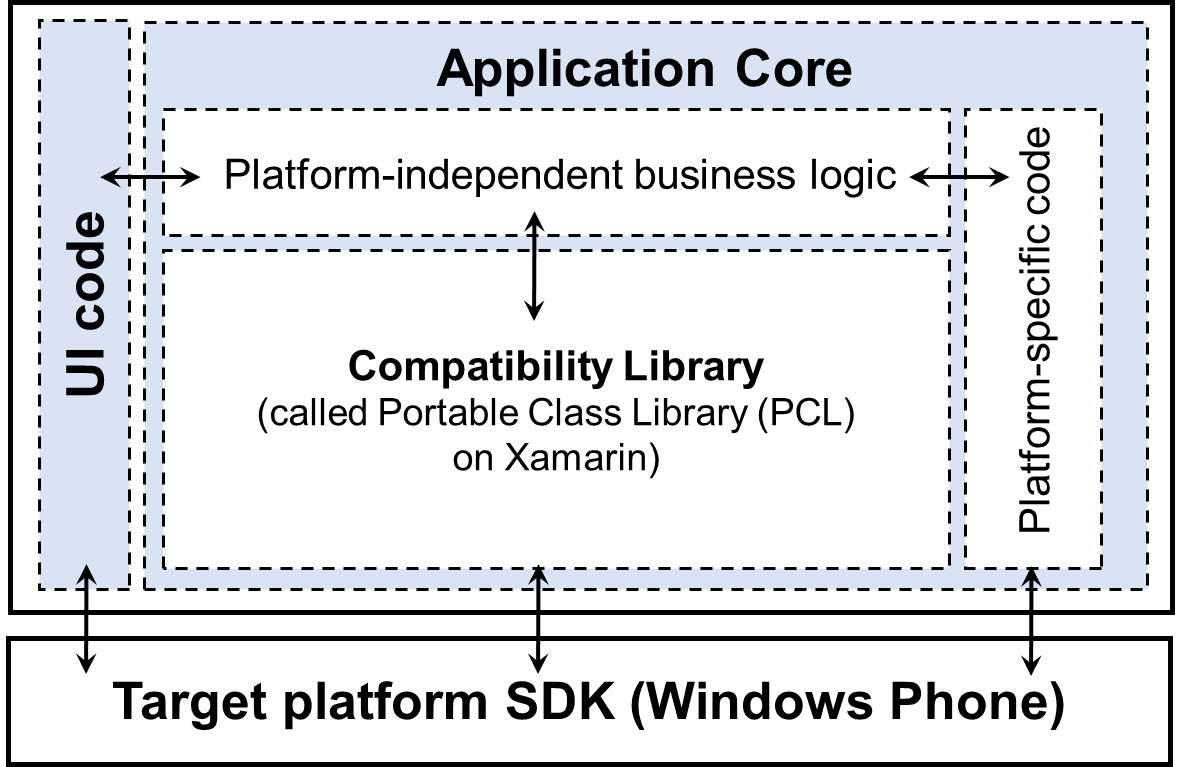
\includegraphics[keepaspectratio=true,width=0.45\textwidth]{figures/appstruct.png}
\mycaption{Structure of a cross-platform app written using Xamarin.}
{\label{figure:appstruct}}
\end{figure}

Xamarin aims to provide support to developers to minimize the amount of
platform-specific code that is needed to port an app across platforms.  To
achieve this goal, one of the main components of the core of a Xamarin-based
app are cross-platform compatibility libraries, also called \textit{portable
class libraries, or PCLs} in Xamarin, a technology originally developed by
Microsoft. On Visual Studio and other Microsoft environments, a PCL is a
special type of a project that allows developers to write code and produce
libraries that can be shared across multiple platforms, such as iOS, Android,
and Windows Phone. To support this, PCLs export an interface of methods and
properties that are portable across platforms, and developers program to this
interface. The app developer encodes platform-independent business logic by
programming to this interface. The PCL provides forwarding stubs that ensures
that calls to methods or property accesses are routed to the correct underlying
platform libraries at runtime.  The developer of the PCL typically identifies
the interface by choosing a set of target platforms that the PCL will support.
Because different platforms provide implementations of differing subsets of the
base \code{.NET} class library, the PCL interface is typically restricted to
the common \code{.NET} functionality that is supported by all the target
platforms. 

PCLs play a key role in Xamarin because they serve as the compatibility layer
between two different platforms. As previously mentioned, about Xamarin's
BugZilla database lists about 7,100 that are directly or indirectly related to
PCL.  Despite the functionality provided by the PCLs, some platform-dependent
business logic may be necessary in the application core.  For example, PCLs are
still in active development, and if the app developer wishes to use features
that are not currently supported by the PCL, he has to do so by writing
platform-specific code, called \textit{shared assets} on Xamarin. It is
possible to write this code once and compile it for all desired target
platforms using compiler or pre-processor directives (\eg~code specific to
Android or iOS would be guarded using a directive such as \code{\#ifdef
ANDROID} or \code{\#ifdef iOS}, respectively).  Naturally, the goal of projects
such as Xamarin is to increase the coverage provided by their PCLs, so as to
minimize the amount of code that must be written as shared asset projects.

In addition to the application core, the app also includes UI code. Currently,
UI code is largely platform-specific because UI elements, \eg~the look and feel
of buttons and widgets, are customized to specific mobile platforms.
Nevertheless, there are ongoing efforts such as \code{Xamarin.Forms} to even
minimize the amount of platform-specific UI code.

% \todo{How many methods supported in Xamarin's PCLs? What fraction of the .NET
% API still not supported?}

In this paper, we are primarily concerned with testing the functionality of the
PCLs on Xamarin that provide support for platform-independent app code.
Therefore, the test cases generated by \tool\ only target the PCL interface.
Our test cases do not directly target the platform-specific UI code. However,
note that many aspects of the layout and functionality of the UI are controlled
by the business logic, which interacts with the target platform's SDK via the
PCLs.  Therefore, by testing the functionality of the PCLs, we indirectly test
the overall functionality of the app's execution on the target platform
(including its UI).

\section{Design of \TOOL}
\label{section:design}

\tool\ aims to find bugs in Xamarin by generating apps, executing these apps on
Windows Phone and Android, and looking for inconsistencies in them. Thus,
\tool's design consists of two parts, the test case generator and the
inconsistency checker.

\myparagraph{Test Case Generation}
%
\tool\ generates test cases that exercise the programming API used by Windows
Phone developers. As illustrated in \figref{section:example}, each test case is
a sequence of method calls to this API. The arguments to these calls are either
values with primitive data types, or references to objects constructed and
modified by method calls appearing earlier in the sequence. The main challenge
is to generate meaningful method sequences that are also effective, \ie~the
test case generator should be able to elicit error cases in Xamarin without
generating too many test cases.

This problem has been investigated in the past in the context of generating
unit tests for object-oriented programs, and tools such as
JCrasher~\cite{jcrasher}
and Randoop~\cite{randoop:icse07} implement such test case generation. In
particular, Randoop uses a \textit{feedback-directed approach} to random test
generation and is the basis for \tool's test generator as well. We now briefly
describe Randoop's (and therefore \tool's) approach to test generation.

The test generator accepts as input a list of classes to be tested, a set of
filters and contracts (which are sanity checks to be performed), and a timeout.
Intuitively, the test generation algorithm iteratively ``grows'' method
sequences from previously-generated shorter sequences. Suppose that the test
generator has already generated a set of method sequences as valid test cases.
During each iteration, the test generator picks a method \code{m(T$_1$,
$\ldots$, T$_n$)} at random from the list of classes provided to it as input,
and ``extends'' the existing method sequences with a call to \code{m} (\eg~one
way to ``extend'' is to append \code{m} to the end of the sequence). If the
parameters of \code{m} are all of primitive type, then the test generator
randomly selects the values of these parameters from a pool of acceptable
values. If the parameter is a reference to an object, then the test generator
uses an object of suitable type created by a method in the sequence that
\code{m} just extended (or passes a \textsc{null} reference). \tool\ then wraps
this method sequence with template code to serialize data structures and to
catch exceptions, as shown in the examples from \sectref{section:example}, to
produce the test cases.

The test generator then executes the newly-generated test sequences looking for
violations of filters and contracts. These are sanity checks that look for
common error cases, such as test cases that throw an exception, or those that
violate certain invariants (\eg~\code{o.equals(o)} not returning \textsc{true}).
Test sequences that violate these sanity checks are discarded, and the
remaining test cases are added to the set of valid test cases, to be extended
in future iterations.  This process continues till the specified timeout has
expired.  This iterative approach is key to generating effective test cases. It
ensures that every prefix of a valid test sequence is also valid, and that test
sequences that violate simple sanity conditions (\eg~those that throw an
exception) are never extended.

\myparagraph{Serializing State and Checking Inconsistencies}
%
For the test cases generated using the approach above, \tool\ produces a pair
of apps for Windows Phone and Android. It executes them atop these platforms to
observe inconsistent behavior. We now discuss the design of the serializer,
which helps identify inconsistencies when both apps return \textsc{success},
\ie~the first case in \figref{table:inconsistency-sources}. The other two cases
are straightforward and we do not discuss them further.

The serializer recursively traverses object references to create serialized
representations. Intuitively, a serialized representation is a set of
(\textsf{key}, \textsf{value}) pairs. The \textsf{key} is the name of a public
field of the object. For fields of primitive type (\eg~\code{bool}, \code{int},
\code{String}), the \textsf{value} is simply the actual value of the field. For
fields that are themselves object references, the value is a serialized
representation of that object. The example below shows the serialized
representation of a linked list with two entries. The \code{data} field of the
entries store \code{1} and \code{2}, respectively.
%
$$
\{
	(``\code{data}", \code{1}),
	(``\code{next}", \{(``\code{data}", \code{2}), 
	                   (``\code{next}", \textsc{null})
	                 \})
\}
$$

\tool's serializer uses the \code{Json.NET}~\cite{jsonnet} library, which
optionally supports the ability to serialize cyclic data structures. It does so
by keeping track of object references using an additional identifier. However,
in our experience, the random test cases that we generate do not produce cyclic
heap data structures. We therefore did not enable support for serializing
cyclic data structures in our prototype, and the serialized object
representations are tree-structured as a result. Note that in the unlikely case
that a test case does produce a cyclic data structure, our serializer would
infinitely loop---a situation we have not encountered to date in our
experiments.

\tool\ identifies inconsistencies by comparing serialized representations of
objects on the home and target platforms. Comparison proceeds recursively in a
bottom-up fashion. All the (\textsf{key}, \textsf{value}) pairs storing
primitive types must match, and the tree-structure of the serialized
representation must be the same, \ie~the same \textsf{key}s on both platforms
at each level of the tree. Any mismatches indicate inconsistent state. In most
of the bugs that we found, the mismatches were because the \textsf{value}s
diverged (\eg~the complex number example in \figref{figure:inconsist-eg}).
However, we also found cases where the fields in the objects were different on
Windows Phone and Android because a field that was declared to be \code{public}
on Windows Phone was a \code{private} field in Android, and therefore not
listed in the serialized representation. 

As previously discussed, the feedback-directed approach to test case generation
does not extend any method sequences that violate its filters and contracts,
\eg~sequences that throw an exception when executed. While Randoop was
originally designed for unit-testing object-oriented programs, \tool\ extends
it for cross-platform differential testing. For practical reasons described in
\sectref{section:implementation}, \tool\ first executes the test case generator
on one platform, where it uses the iterative approach to output test cases.  It
then executes these test cases on the target platform (Android). Thus, \tool's
test cases also preserve the property that only non-exception-generating test
cases are extended in the iterative process. 

However, because \tool\ generates all the test cases on the home platform
before executing them on the target platform, even those test cases that return
\textsc{success} but produce inconsistent serialized state across the two
platforms are extended during test generation. As a result, it is possible that
multiple test cases produced by \tool\ may report the same inconsistency.

\myparagraph{Discussion}
%
Differential testing offers an attractive property. If a test case is executed
on two API implementations with the same initial state, any inconsistency in
the final states indicates a problem in at least one of the API
implementations. That is, differential testing \textit{does not produce false
positives.}

However, in practice, it is possible that an inconsistency does not always
correspond to a problem. In our experiments, we found that such a situation
could arise because of any one of a small number of reasons.  First, some API
methods, such as those from \code{System.Random} and \code{System.Time}, invoke
platform-specific features and return different values when invoked on
different platforms. For example, the \code{System.Net.Cookie()} constructor
initializes \code{Cookie.TimeStamp} with the current system time. Unless the
emulation environments that run the apps for both the home and target platforms
are synchronized, this call will return different values.  Second, for some
methods, such as \code{Object.GetHashCode}, the documentation specifies that
the behavior of the method varies across platforms. That is, the
\code{HashCode} of an object can be different on the home and target platforms
even if the serialized representations of the object are the same on both
platforms. A third source of false positives was because the Mono runtime
included in a Xamarin-produced Android app uses Mono Assemblies as its
libraries. These libraries have different metadata information than their
Windows Phone counterparts, and any calls that access this metadata will result
in inconsistent serialized state.

\begin{figure}[t!]
\centering
\scriptsize
\begin{tabular}{|l@{~|~}p{0.25\textwidth}|}
\hline
\multicolumn{2}{|c|}
{\textbf{Filtered classes:} All methods/variables of this class filtered.}\\
\hline
\code{System.Random} & 
	Members return random values\\
\hline
\hline
\multicolumn{2}{|c|}
{\textbf{Filtered methods:} Methods cannot appear in test cases.}\\
\hline
\code{System.Type GetType()} & 
	Return value may include information from the underlying C\# assembly, which
	is not uniform across platforms\\
\code{System.Int32 GetHashCode()} & 
	Documentation specifies that hash code of similar objects need not be similar across platforms\\
\hline
\hline
\multicolumn{2}{|c|}
{\textbf{Filtered constructors:} Constructor cannot appear in test cases.}\\
\hline
\code{System.Xml.UniqueId()} & 
	Returns a unique GUID, which is not guaranteed to be consistent across
	platforms\\
\hline
\hline
\multicolumn{2}{|c|}
{\textbf{Filtered fields/properties:} Cannot be accessed in test cases.}\\
\hline
\code{System.Net.Cookie.TimeStamp} & Value relies on system time at object creation\\
\code{System.DateTimeOffset.Now}   & Value relies on system time\\
\code{System.DateTimeOffset.UtcNow} & Value relies on system time\\
\code{System.DateTime.Now}         & Value relies on system time\\
\code{System.DateTime.UtcNow}      & Value relies on system time\\
\code{System.DateTime.Today}       & Value relies on system time\\
\code{System.Exception.HResult}    & Value identifies an exception, but
documentation is not conclusive about whether value is consistent across
platforms\\
\hline
\end{tabular}
\mycaption{Filters used by \tool\ to avoid generating test cases that produce false positives.}
{\label{figure:filters}}
\end{figure}

Fortunately, it is relatively easy to filter out test cases that can
potentially lead to such false positives. We simply integrate filters that
prevent the test generator from producing method sequences that contain method
calls or field references that can potentially trigger such false positives.
Thus, with just a few filters to eliminate the causes above (see
\figref{figure:filters}), we were able to eliminate false positives, thereby
ensuring that all inconsistencies reported by \tool\ indeed correspond to real
bugs.  Note, however, that as with most other testing tools, our differential
testing approach does have false negatives---\ie~it is not guaranteed to find
all possible inconsistencies.

\section{Practical Considerations}
\label{section:implementation}

In this section, we discuss a few practical issues that we had to address as we
built \tool.

\myparagraphnodot{Where to Generate Test Cases?} 
%
The first practical consideration that we addressed was the question of which
platform to use to execute our test generator. One possibility was to use
Windows Phone, Xamarin's home platform. This requires us to execute \tool\
directly on a device or emulator running Windows Phone. However, we found that
the environment on such devices and emulators was somewhat awkward to use
during active development of \tool, \eg~to debug any issues that arose. We
therefore decided to develop and execute \tool\ on a desktop version of Windows
(8.1). Our hypothesis was that the desktop and phone versions would be largely
similar because they use the same \code{.NET} code base, and as a result, we
could use the desktop to generate the test cases and execute them as apps on
Windows Phone and Android devices.

This approach eased development of \tool, and for the most part our hypothesis
about the equivalence of the desktop and phone version of Windows was correct.
However, we found (and reported to Microsoft) 
%\cite{nader:connect:1} 
a case where the desktop and phone versions diverged in their semantics. In
particular, the public property \code{CurrencyDecimalDigits} of the class
\code{System.Globalization.NumberFormatInfo} is required to be a read-only
field according to MSDN documentation. While the read-only property holds in
the desktop version, the property is mutable in the Windows Phone version. We
also found, using differential testing against Android, a case where both the
desktop and phone version of Windows incorrectly implement the documented
semantics for a given property, while Android's implementation followed
Microsoft's documentation. In particular, the property \code{WebName} of
\code{System.Text.Encoding.BigEndianUnicode} must have the value
\code{UTF-FFFE} according to Microsoft's documentation, but the desktop and
phone version of Windows return \code{UTF-16BE}.

\myparagraph{PCLs and Test Generation}
%
A second issue that we had to address was the integration of \tool's test
generator and PCLs.  As previously discussed, \tool's test generator produces
test cases for a given input set of classes. It uses reflection to identify
public methods from those classes, the data types of their arguments and the
other properties of these classes, and uses this information in its test
generation algorithm.

However, PCLs pose a unique problem when used with \tool's test generator.
Recall that PCLs define the interface against which developers can build their
applications without concerning themselves with cross-platform portability
issues. PCLs enable this feature by transparently acting as forwarders---they
route calls from the application layer to the corresponding library in the
platform on which the application is loaded. Thus, PCLs usually do not contain
any of the executable code of the classes for which they act as an interface,
and merely contain forwarding stub code. As a result of this feature, when
\tool's test generator is provided with a set of PCL classes as input, it is
unable to use reflection to fetch the complete set of public methods, data
types and properties of the classes for which the PCL acts as a forwarder.

To address this issue, we had to extract the information required by \tool's
test generator by loading PCLs in a non-executable \textit{reflection-only}
mode. In this mode, PCLs are not executable, but can be queried using
reflection and return metadata by accessing the corresponding classes on the
platform. We then re-load the PCLs in executable mode, and use the metadata to
iteratively generate and execute test cases.

\myparagraphnodot{How to Package Test Cases?} 
%
Finally, we also had to address the issue of how to package up the test cases
for execution on the Windows Phone and Android platforms. Each test case is
packaged as a separate class that can be instantiated and executed. As
discussed above, we run the iterative test generation algorithm on the desktop
version of Windows. As a result, we have all the test cases available for batch
execution on the mobile platforms. 

\begin{figure}[t!]
\centering
\begin{tabular}{cc}
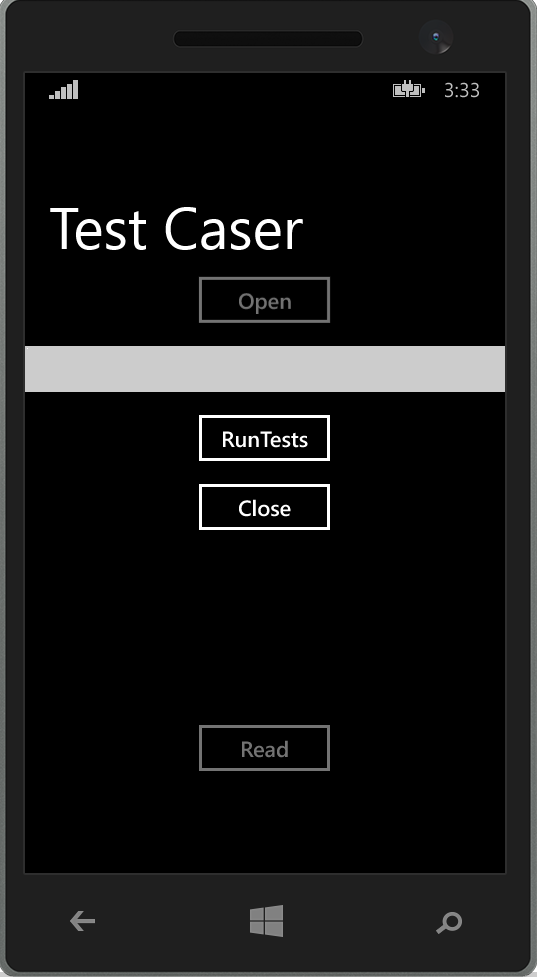
\includegraphics[keepaspectratio=true,height=5cm]{figures/windows.png} &
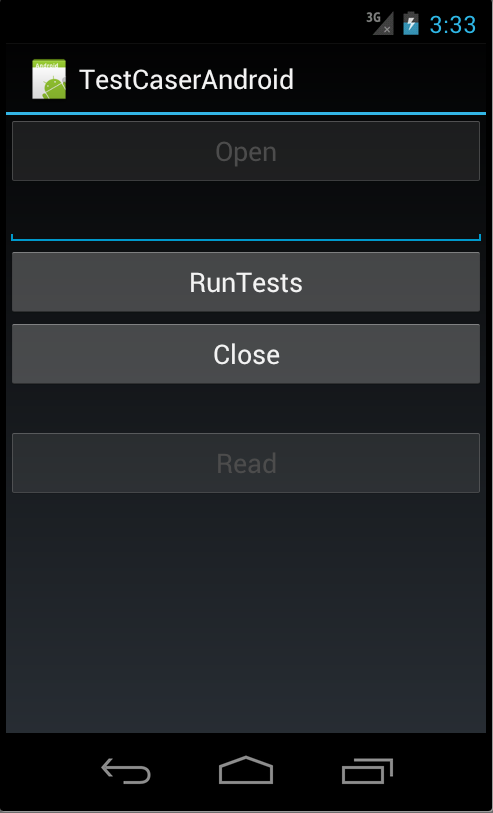
\includegraphics[keepaspectratio=true,height=5cm]{figures/android.png}\\
{\bf \small (a) Windows Phone version} &
{\bf \small (b) Android version}
\end{tabular}
\mycaption{Screenshots showing the UIs of the test case apps on Windows Phone
and Android.}{\label{figure:screenshot-testcase}}
\end{figure}

We package all the test cases into a single app each for execution on the two
mobile platforms. Both Windows Phone and Android require apps to define a UI.
We wrote this UI and the code to interface with the file system (to store the
logs generated when test cases are executed) within a  platform-specific
presentation layer, and packaged up the test cases as platform independent code
to be cross-compiled by Visual Studio and Xamarin. All the test cases generated
by \tool\ can be invoked at the press of a single button on the app.
\figref{figure:screenshot-testcase} shows the UIs of the Windows Phone and
Android versions of these apps. The UIs of these apps look rather
different---each app uses buttons and icons unique to the corresponding mobile
platform. However, because our test cases focus only on the
platform-independent PCL classes, the differences in the UI state do not
manifest as divergent state (and therefore as inconsistencies) during the
execution of the test-cases.


\section{Evaluation}
\label{section:evaluation}

In evaluating \tool, our main goals were to demonstrate the flexibility of
\tool\ by showing that it can check compliance against a variety of policies,
and understand the performance costs of various components of \tool.

Our setup consisted of running OpenSGX atop of Ubuntu 14.04 on a physical
machine  equipped with an Intel Core i5 CPU and 16GB of memory. We use clang
and llvm version-3.6 to compile and instrument many real world applications to
run within enclaves: Nginx (an HTTP server), Memcached (a popular key-value
store), Netperf (a networking benchmark), otp-gen (a password generator),
graph-500 (a graph data benchmark) and two SPEC benchmarks (401.bzip2 and
429.mcf). In all experiments, all the applications are compiled as position
independent executables and are statically linked. To keep the size of the
executables small all applications are linked against musl-libc~\cite{musllibc}
instead of GNU libc~\cite{gnulibc}. \figref{table:tcb} shows the lines of code
of all the components of \tool's implementation. In the following sections, we
describe the performance costs of three policy modules that we implemented in
\tool. For each benchmark, we assume that the benchmark executes within the
enclave, and we evaluate the cost of \tool\ as it loads the benchmark within
the enclave for execution, and checks for policy compliance.

\begin{figure}[t!]
\centering
\footnotesize{
\begin{tabular}{|p{0.35\textwidth}|r|}
\hline
 \bf Components                    & \bf LOC \\
\hline
Code Provisioning & 270\\
\hline
Loading and Relocating & 188\\
\hline
Checking Executables linked against musl-libc & 1,949\\
\hline
Checking Executables Compiled with Stack Protection & 109\\
\hline
Checking Executables Containing Indirect Function-Call Checks & 129\\
\hline
Client's side program & 349\\
\hline
Musl-libc & 90,728\\
\hline
Lib crypto (openssl) & 287,985\\
\hline
Lib ssl (openssl) & 63,566\\
\hline
Total & 453,349\\
\hline
\end{tabular}}
\mycaption{Sizes of various components of \tool. Some of these components
(\eg~the cryptographic libraries) are part of the default loader in all enclave
implementations.}
{\label{table:tcb}}
\indent\vspace{-0.5cm}
\end{figure}

\myparagraph{Compliance for Library Linking.}
%
When a cloud provider allows a client to run code on its platform, it often
expects the client to run a particular version of the code. For example, the
cloud provider may require that the client execute a version of the code that
has been patched with the latest security updates. As a special case of this,
the cloud provider may wish to check whether the client's code has been linked
against specific versions of certain libraries. For example, the cloud provider
may wish to ensure that if the client's code uses OpenSSL, then the version of
OpenSSL that is used is free of the vulnerability that caused the HeartBleed
exploit. As another example, consider
\code{/CONFIDENTIAL}~\cite{moatplus:pldi16}, a library that ensures that
enclave code satisfies certain information-flow confinement properties,
\ie~enclave code that is linked against this library will not accidentally leak
sensitive information. To prevent liability issues arising from any accidental
data leaks in the client's code, the cloud provider may wish to ensure that the
client's code is linked with the \code{/CONFIDENTIAL} library. 

To illustrate the power of \tool\ at enforcing such library-linking policies,
we implemented a policy module that verifies whether an executable is linked
against musl-libc~\cite{musllibc} version 1.0.5. To perform this check, we
first generate the SHA-256 hashes of all the functions of musl-libc v1.0.5.
For enforcement, the policy module iterates through the instruction buffer of
the code to be loaded in the enclave, and looks for all direct function calls.
For each direct function call, the policy check computes the target of the call
and then looks up the symbol hash table to get the function name of the target.
If the target does not exist in the symbol hash table the check will mark the
function call as invalid; otherwise, it will compute the SHA-256 hash of all
the instructions of the function. Specifically, the policy module sequentially reads instructions starting from 
the computed target address and stops when it comes across an instruction that 
is at the beginning of another function. The policy module relies on the symbol hash
table to identify whether an instruction address is at the beginning of a function. The policy check next compares the hash of the
function in the executable with its hash in musl-libc. If the two hashes do not
match, the client has not provided the required musl-libc; otherwise, the
policy check continues with the next iteration until it reaches the end of the
instruction buffer.

\begin{figure}[t]
\centering
\scriptsize{
\begin{tabular}{|l|r|r|r|p{0.1\linewidth}|}
\hline
 \bf Benchmark & 
     \bf \#Inst. & 
    \bf Disassembly & 
    \bf Policy Checking & 
    \bf Loading and Relocation\\
\hline
Nginx & 262,228 & 694,405,019 & 1,307,411,662 & 128,696\\
\hline
401.bzip2 & 24,112 & 34,071,240 & 148,922,245 & 4,239\\
\hline
Graph-500 & 100,411 & 140,307,017 & 246,669,796 & 4,582\\
\hline
429.mcf & 12,903 & 18,242,127 & 123,895,553 & 4,363\\
\hline
Memcached & 71,437 & 137,372,517 & 489,914,732 & 8,115\\
\hline
Netperf & 51,403 & 90,616,563 & 367,356,878 & 18,090\\
\hline
Otp-gen & 28,125 & 42,823,024 & 198,587,525 & 5,388\\
\hline
\end{tabular}}
\mycaption{Performance of \tool\ to check the \textit{Library-linking} policy.
Here \tool\ checks whether each benchmark has been linked against musl-libc.
The figure shows the size of each benchmark, measured as the number of
instructions in the code to be loaded in the enclave, and the time taken to
execute each step of \tool, reported as CPU cycles. Wall-clock time can be
obtained by multiplying CPU clock cycles with the clock cycle time. A CPU with
a clock rate of 3.5GHz as used in our experiments has 1/3.5 nanoseconds cycle
time. Therefore, the 694,405,019 cycles it takes to disassemble Nginx, for
example, consumes 198.4 milliseconds.}
{\label{table:checkinglinkedlib}}
\indent\vspace{-0.5cm}
\end{figure}

To compute the performance cost, we adopt the approach suggested in the OpenSGX
paper~\cite{opensgx:ndss16} and assume that each SGX instruction takes 10K CPU
cycles and non-SGX instructions run at native speed within the enclave.  We
leverage OpenSGX's performance counter and QEMU's instruction count~\cite{qemu}
to count SGX and non-SGX instructions. We calculate the CPU cycles of non-SGX
instructions by measuring the instructions per cycle by executing the loader
natively without OpenSGX.  \figref{table:checkinglinkedlib} presents the
results of our experiments when running this policy check against different
benchmarks.  

\renewcommand{\baselinestretch}{0.9}
\myparagraph{Compliance for Stack Protection.}
%
Given the prevalence of buffer overflow vulnerabilities in low-level code, a
number of modern compilers now give the option of emitting extra code to
protect loads and stores to memory locations. Clang's \code{-fstack-protector}
flag lets the LLVM compiler add a guard variable when a function starts and
checks the variable when a function exits. For instance, when compiled with the
flag, the following extra code is emitted:

\begin{center}
\footnotesize{
\begin{tabular}{ll}
\code{19311:} & \code{mov    \%fs:0x28, \%rax}\\
\code{1931a:} & \code{mov    \%rax, (\%rsp)}\\
\code{193fe:} & \code{mov    \%fs:0x28, \%rax}\\
\code{19407:} & \code{cmp    (\%rsp), \%rax}\\
\code{1940b:} & \code{jne    1941f}\\
\code{1941f:} & \code{callq  8d5bf <\_\_stack\_chk\_fail>}\\
\end{tabular}}
\end{center}

The two instructions at addresses \code{193fe} and \code{19407} check if the
variable at the top of the stack is the same as the variable at
\code{\%fs:0x28}. If the values do not match, control will be transfered to the
\code{\_\_stack\_chk\_fail} function.

Clang also provides the \code{-fstack-protector-all} option which is similar to
\code{-fstack-protector} except that \textit{all} functions are protected. To
check whether an executable is compiled with this flag, the policy module
iterates through the instruction buffer and identifies the start of a function
using the symbol hash table. Within each function, the policy check looks for
instructions that affect the stack's variables (\eg~\code{mov \%rax,(\%rsp)} in
the above example). It then identifies the source operand of the instruction
(\code{\%rax}) and figures out the value of the source operand (\code{mov
\%fs:0x28,\%rax}).  As a next step, it checks if the function contains a
\code{cmp} instruction with the source and destination are the stack's variable
and the previous source operand, respectively. It also has to check that just
preceding the \code{cmp} instruction, there is an instruction that computes the
original value of the source operand (\code{mov \%fs:0x28,\%rax}). Finally, the
policy looks for the \code{jne} and \code{callq} instructions. It computes the
target of the \code{callq} instruction and checks the symbol hash table to
verify that the target corresponds to the the \code{\_\_stack\_chk\_fail}
function.

\begin{figure}[t]
\centering
\scriptsize{
\begin{tabular}{|l|r|r|r|p{0.1\linewidth}|}
\hline
 \bf Benchmark         & 
     \bf \#Inst. & 
    \bf Disassembly & 
    \bf Policy Checking & 
    \bf Loading and Relocation\\
\hline
Nginx & 271,106 & 719,360,640 & 713,772,098 & 128,662\\
\hline
401.bzip2 & 24,226 & 34,292,136 & 862,023,613 & 4,206\\
\hline
Graph-500 & 100,488 & 140,588,361 & 195,218,892 & 4,548\\
\hline
429.mcf & 12,985 & 18,288,921 & 31,459,881 & 4,330\\
\hline
Memcached & 71,677 & 137,877,497 & 325,442,403 & 8,081\\
\hline
Netperf & 51,868 & 91,577,335 & 183,274,713 & 18,057\\
\hline
Otp-gen & 28,217 & 43,053,386 & 217,302,816 & 5,355\\
\hline
\end{tabular}}
\mycaption{Performance of \tool\ to check the \textit{Stack protection}
policy.  As before, for performance numbers, we report the CPU cycles.}
{\label{table:checkingstackprotection}}
\indent\vspace{-0.5cm}
\end{figure}

Of course, our implementation of \tool's policy module is customized for
Clang's stack protection instrumentation as emitted by the
\code{-fstack-protector} flag. It can easily be customized to check stack
protection instrumentation inserted by other tools, such as Google's
AddressSanitizer~\cite{google:asan:usenix:2012}, LLVM
SoftBound~\cite{softbound:pldi09}, etc.  \figref{table:checkingstackprotection}
presents the results of our experiments when running this policy check against
different benchmarks executing in enclaves.

\myparagraph{Restricting Indirect Function Calls.}
%
Protecting applications against control-flow hijacking attacks is one of the
emerging concern due to the fact that attackers have recently focused on taking
advantage of heap-based corruptions to overwrite function pointers to change
the flow of a program. Control-flow Integrity (CFI)is a measure that guards
against these attacks by restricting the targets of indirect control transfers
to a set of precomputed locations.

We implemented a policy check to verify that executables are compiled with
indirect function-call checks as proposed in recent work by Google
(IFCC)~\cite{edgecfi:sec14}. IFCC protects indirect calls by generating
instrumentation for the targets of indirect calls. It adds code at indirect
call sites to ensure that function pointers point to a jump table entry. For
example, the LLVM implementation of IFCC emits the following code for an
indirect function call:

\begin{center}
\footnotesize{
\begin{tabular}{ll}
\code{1b459:} & \code{lea  0x85c70(\%rip), \%rax} \\
              & \code{\#<\_\_llvm\_\#jump\_instr\_table\_0\_1>}\\
\code{1b460:} & \code{sub  \%eax, \%ecx}\\
\code{1b462:} & \code{and  \$0x1ff8, \%rcx}\\
\code{1b469:} & \code{add  \%rax, \%rcx}\\
\code{1b475:} & \code{callq *\%rcx}\\
\end{tabular}}
\end{center}

To instrument executables with these checks, we use the LLVM/clang
toolchain enhanced with the IFCC patch~\cite{llvmforwardedgecfi}. To check
whether an executable is compiled with IFCC checks, \tool's policy module first
figures out the range of the jump table by relying on the fact that all jump
table entries have the following format:

\begin{center}
\footnotesize{
\begin{tabular}{ll}
\multicolumn{2}{l}{\code{a19d0 <\_\_llvm\_jump\_instr\_table\_0\_289>:}}\\
\code{a19d0:} & \code{~~~~jmpq   41090 <ngx\_execute\_proc>}\\
\code{a19d5:} & \code{~~~~nopl   (\%rax)}\\
\end{tabular}}
\end{center}

\begin{figure}[t]
\centering
\scriptsize{
\begin{tabular}{|l|r|r|r|p{0.1\linewidth}|}
\hline
 \bf Benchmark         & 
    \bf \#Inst. & 
    \bf Disassembly & 
    \bf Policy Checking & 
    \bf Loading and Relocation\\
\hline
Nginx & 267,669 & 821,734,999 & 20,843,253 & 128,668\\
\hline
401.bzip2 & 24,201 & 34,235,817 & 1,751,276 & 4,206\\
\hline
Graph-500 & 100,424 & 140,429,738 & 7,014,913 & 4,548\\
\hline
429.mcf & 12,903 & 18,242,127 & 1,177,429 & 4,330\\
\hline
Memcached & 71,508 & 138,231,446 & 5,301,168 & 8,081\\
\hline
Netperf & 51,431 & 91,161,601 & 3,775,318 & 18,057\\
\hline
Otp-gen & 28,132 & 42,829,680 & 2,334,847 & 5,355\\
\hline
\end{tabular}}
\mycaption{Performance of \tool\ to check the \textit{Indirect Function-Call}
policy.  As before, for performance numbers, we report the CPU cycles.}
{\label{table:checkingindirectfunccall}}
\indent\vspace{-0.4cm}
\end{figure}

\tool's policy module for this check iterates through the instruction buffer
and looking for indirect function calls. It then verifies that before the
indirect function calls, there is a sequence of instructions \code{lea},
\code{sub}, \code{and} and \code{add}, with data dependence between registers
as shown in the code snippet above. It then computes the target of the indirect
call and verifies that the target is within the range of the jump table.
\figref{table:checkingindirectfunccall} presents the results of our experiments
when running this policy check against different benchmarks.

\mysection{Related Work and Design Alternatives}
\label{section:related}

\myparagraph{TrustZone Support}
%
A number of projects have used TrustZone to build novel security applications.
TrustDump~\cite{trustdump:esorics14} is a TrustZone-based mechanism to reliably
acquire memory pages from the normal world of a device (Android
LiME~\cite{lime} and similar tools~\cite{dmd,ddms,recoverymode} do so too, but
without the security offered by TrustZone).  While similar in spirit to remote
reads, TrustDump's focus is to be an alternative to virtualized memory
introspection solutions for malware detection. Unlike our work, TrustDump is
not concerned with restricted spaces, authenticating the host, or remotely
configuring guest devices.

Samsung Knox~\cite{knox:ccs14} and \textsc{Sprobes}~\cite{sprobes:most14}
leverage TrustZone to protect the normal world in real-time from kernel-level
rootkits. These projects harden the normal world kernel by making it perform a
world switch when it attempts to perform certain sensitive operations to kernel
data. A reference monitor in the secure world checks these operations, thereby
preventing rootkits. In our work, remote reads allow the host to detect
infected devices, but we do not attempt to provide real-time protection from
malware. Our work can also leverage Knox to enhance the security of the normal
world (\sectref{section:threat}).

TrustZone has also been used to improve the security of user applications.
Microsoft's TLR~\cite{tlr:asplos14} and Nokia's ObC~\cite{obc:asiaccs09} use
TrustZone to provide a secure execution environment for user apps, even in the
presence of a compromised kernel. Other applications include ensuring
trustworthy sensor readings from peripherals~\cite{tenor:mobisys12} and
securing mobile payments~\cite{proxama}.

\myparagraph{Enterprise Security} With the growing ``bring your own device''
(BYOD) trend, a number of projects have developed enterprise security solutions
that enable multiple persona
(\eg~\cite{asm:sec14,flaskdroid:sec13,cells:sosp11}) or enforce mandatory
access control policies on smart devices
(\eg~\cite{deepdroid:ndss15,seandroid:ndss13,flaskdroid:sec13,asm:sec14}).
Prior work has also explored context-based access control and techniques for
restricted space objects to push usage policies onto guest devices
(\eg~\cite{saint:acsac09,Covington2002,conxsense:asiaccs14,worlddriven:ccs14,blindspot:2009,markit:upside14}).

These projects tend to use one of two techniques. One is to require guest
devices to run a software stack enhanced with a policy enforcement mechanism.
For instance, ASM~\cite{asm:sec14} introduces a set of security hooks in
Android, which consult a security policy (installed as an app) that can be used
to create multiple persona on a device. Each persona is customized with a view
of apps and peripherals that it can use. Another approach is to require
virtualized guest devices
\cite{cells:sosp11,cox:hotmobile07,vmwareverizon,kvmarm:asplos14}. In this
approach, a trusted hypervisor on the guest device enforces isolation between
VMs implementing different persona.

The main benefit of these techniques over our work is the greater app-level
control that they provide. For example, they can be used to selectively block
sensitive audio and blur faces by directly applying policies to the
corresponding user apps~\cite{worlddriven:ccs14,ar:sec13}. These techniques
are able to do so because they have a level of semantic visibility into
app-level behavior that is difficult to achieve at the level of raw memory
operations.

On the other hand, our approach enjoys two main benefits over prior work.
First, our approach simplifies the design of the trusted policy-enforcing code
that runs on guest devices to a TCB of just a few thousand lines of code. In
contrast, security-enhanced OSes and virtualized solutions required hundreds of
thousands of lines of trusted policy-enforcement code to execute on guest
devices.  Prior research has investigated ways to reduce the TCB, \eg~by
creating small hypervisors~\cite{nova:eurosys09}. However, the extent to which
such work on small hypervisors applies to smart devices is unclear, given that
any such hypervisor must support a variety of different virtualization modes,
guest quirks, and hardware features on a diverse set of personal devices.

The second benefit of our approach is that it provides security guarantees that
are rooted in trusted hardware. Prior projects have generally trusted guest
devices to correctly implement the host's policies. This trust can easily be
violated by a guest running a maliciously-modified OS or hypervisor.  It is
also not possible for a host to obtain guarantees that the policy was enforced
for the duration of the guest's stay in the restricted space. We leverage the
TrustZone to offer such guarantees using verification tokens and REM-suspend.

\myparagraph{Other Hardware Interfaces}
%
Hardware interfaces for remote memory operations were originally investigated
for the server world to perform remote DMA as a means to bypass the performance
overheads of the TCP/IP stack~\cite{mellanox,infiniband}.  This work has since
been repurposed to perform kernel malware detection~\cite{copilot:sec04} and
remote repair~\cite{backdoor:icac04}. These systems use a PCI-based
co-processor on guests via which the host can remotely transfer and modify
memory pages on the guest.

On personal devices, the closest equivalent to such a hardware interface is the
IEEE 1394 (Firewire), which is available on some laptops. However, it is not
currently available on smaller form-factor devices.  Another possibility is to
use the JTAG interface~\cite{jtag}, which allows read/write access to memory
and CPU registers via a few dedicated pins on the chipset.  However, the JTAG
is primarily used for debugging and is not easily accessible on consumer
devices.  One drawback of repurposing these hardware interfaces is that they
cannot authenticate the credentials of the host that initiates the memory
operation. Moreover, to use these hardware interfaces on guest devices, the
host needs physical access to plug into them.  Thus, these interfaces are best
used when the guest can physically authenticate the host and trust it to be
benign.


% \myparagraph{App Security}
% 
% It is now well-known that many popular apps exfiltrate sensitive user data
% from smart devices~\cite{taintdroid:osdi10}. Moreover, a significant fraction
% of apps (on Android) are over-privileged~\cite{stowaway:ccs11,pscout:ccs12}
% and end-users are poor at understanding the meaning of app
% permissions~\cite{ep:ubicomp12,felt:soups12}.  Such apps can leverage the
% increasing array of sensors on modern smart devices in novel and dangerous
% ways~\cite{soundcomber:ndss11,placeraider:ndss13}. These threats will amplify
% in the future as we see an increasing number of augmented reality apps that
% continuously monitor sensor feeds and extract data from the device's
% environment.

% Some projects have attempted to rectify the situation by offering improved
% app permission models~\cite{howtoask:hotsec12} or modifying the execution
% environment on the device to return ``fake'' sensor data to
% apps~\cite{mockdroid:hotmobile10}. However, such techniques are usually
% ineffective when the device itself is compromised (\eg~via kernel rootkits),
% or if the user unintentionally installs a malicious app.  Our work can
% complement these efforts by allowing hosts to control peripherals below the
% app layer. 

% \myparagraph{Hardening Smart Devices}
% 
% Finally, the research community has addressed techniques to harden the
% software stack of smart devices. Samsung Knox~\cite{knox:ccs14}, as
% previously discussed, provides the ability to detect certain classes of
% kernel-level rootkits in real time.  MOCFI~\cite{mocfi:ndss12} enhances the
% mobile OS by enforcing control-flow integrity properties,
% thereby mitigating the effect of attacks such as buffer overflow-based
% exploits.  Airbag~\cite{airbag:ndss14} employs lightweight virtualization to
% isolate user apps and prevent them from infecting the device's firmware or
% leaking sensitive information. At the app level,
% RetroSkeleton~\cite{retro:mobisys13} rewrites Android apps to improve their
% security on commodity devices. These techniques can help improve the
% resilience of smart devices to attack. Our work allows hosts to remotely
% analyze smart devices via remote memory operations and verify that they are
% free of malware infection.


% \myparagraph{Defending from Malware}
% \myparagraph{Context Awareness}



% * Clear difference from SAMSUNG KNOX.
% * List the things that we don't want to do (because SAMSUNG KNOX is our competition)
%     - Intercept critical operations.
%     - They cannot detect memory overflow errors.
%     - Ours is asynchronous, theirs is synchronous.
%     - No writes/uninstalling devices.
% * KNOX is not enforcing any enterprise security policy. Ours is enforcing specific enterprise policies.
% * KNOX checks the integrity of certain kernel memory pages.
%
% Prior work has developed numerous examples of security primitives that use
% remote memory operations. Examples include memory forensics~\cite{}, kernel
% malware detection~\cite{}, and OS repair~\cite{}.  
% However, the bulk of these techniques have usually been developed for
% server-class systems or personal computers with larger form factors, such as
% desktops, that typically use the x86 architecture and where methods to isolate
% the target from the monitor, \ie~virtualization or co-processors, are readily
% available.
%

\section{Conclusion}
\label{section:conclusion}
This paper presents the design and implementation of EnGarde, an enclave inspection library 
that preserves the security benefits offered by the SGX and allows the cloud provider to 
verify the client's SGX-based enclave against a set of policies mutually agreed by the 
cloud provider and the client. In EnGarde, the cloud provider and the client mutually trust 
the inspection library with policy enforcement. EnGarde achieves its goal by using SGX's 
hardware attestation and having an encrypted channel set up between the cloud provider 
and the client. EnGarde only allows the client content to execute if the content follows
mutually agreed policies. We have evaluated the effectiveness of EnGarde by using it to
enforce three popular security policies for various real world applications.




\myparagraph{Acknowledgments.} Funded in part by NSF CNS-1420815 and a 
gift from Microsoft Research India.

%------------------------------------------------------------------------------
%                                  References.
%------------------------------------------------------------------------------
\scriptsize
\bibliographystyle{plain}
\bibliography{references}

\end{document}
